\documentclass[11pt]{article}
\usepackage[margin=1in]{geometry}
\usepackage[T1]{fontenc}
\usepackage{lmodern}
\usepackage{microtype}
\usepackage{booktabs}
\usepackage{graphicx}
\usepackage{amsmath}
\usepackage{enumitem}
\usepackage{xcolor}
\usepackage[hidelinks]{hyperref}
\usepackage{caption}
\captionsetup{font=small,labelfont=bf}
\setlist{itemsep=2pt,topsep=3pt}

\newcommand{\tautwo}{$\tau^2$-bench}
\newcommand{\quoted}[1]{\textit{``#1''}}

\title{\textbf{Garbage In, Refund Out}\\[2pt]
\large When do support agents check contradictory records?}
\author{Raghav Chaudhary}
\date{September 2026}

\begin{document}
\maketitle

\begin{abstract}
A support agent can follow policy while trusting a corrupt record. We plant detectable contradictions in real
\tautwo{} airline and retail data and compare checks tied to actions with checks tied explicitly to yes/no answers.
In an airline single-decision follow-up, Gemini~3.8~Flash wrongfully refused 55/96 corrupted ``no'' records under
``before deciding on a cancellation or refund'', versus 8/96 under ``before telling the customer yes or no''
(paired difference $-49$ percentage points, 95\% bootstrap CI $[-59,-38]$). A refusal-naming instruction gave 0/96;
all three gave 0/96 corrupted payouts. Claude Opus~5.5 made 0/24 wrongful refusals and 0/24 corrupted payouts under
every one of the four wordings (24 fresh bases): no wording effect is measurable at floor. A later preregistered cross-model follow-up (2026-09-28; \texttt{FINDINGS.md}) found the wording effect absent in Claude~Sonnet~5 on 62 new bases (44/62 vs 40/62), partial in Gemini~3.1~Pro, and untestable in GPT-6 (no errors); it also found that checks ran before a ``yes'' and were skipped before a ``no'' in Flash, Pro and Sonnet. This is not a universal
result: a corrected retail-cancel replication gave 0/36 refusals under either wording, and in the earlier
full-conversation study Flash refused 2/8 versus 1/8 in the raw harness output (0/8 under each after a hand recode
that counts flagging without a transfer call as held; a small stress test that may reflect a format effect).
Showing a deterministic airline reconciliation yielded 0/24 bad payouts, 0/24 wrongful refusals and 0/48 clean
control errors; the shown ledger states the mismatch, so this tests acting on a stated mismatch, not checking. A prospectively specified 3,672-decision Flash extension (six wordings, 65 airline bases, two calls per item) found 288/390 airline refusals under action-tied wordings versus 10/390 under answer-tied wordings, but zero refusals under either type in both retail tasks. The prespecified requirement for the same direction in two of three tasks was not met because both retail tasks were at floor (0 refusals under either wording); the retail tasks could not show the effect, so generality beyond this airline task is untested. A further 600-call retail arithmetic analogue used synthetic gift-card balances and produced 0/126 versus 0/126 wrongful refusals; the effort rule was not testable (retail analogue at floor; its `no' path runs through the corrupted number). The analogue does not isolate effort causally. The practical recommendation is to validate both approval and refusal
paths per model and task, and expose deterministic checks with explicit adjustment provenance and counting rules.
\end{abstract}

\section{Problem}

A deployed support agent reads a record, applies the policy, and acts. Benchmarks such as \tautwo{}
\cite{tau2}, the successor to $\tau$-bench \cite{tau}, grade whether the agent follows the policy given the record; they assume the record is right. Real
systems of record are not: migrations, manual edits and buggy writes leave fields that disagree with each other. In
\tautwo{} the payment history is redundant with the rest of the record (airline: payments $=$ fares $\times$
passengers $+$ \$30 per passenger if insured $+$ \$50 per paid bag, which holds on 2,000 of 2,000 reservations;
retail: every order's first payment equals the sum of its items), so a single corrupted field is detectable by
arithmetic the agent can do from what it sees.

We ask three questions a team deploying such an agent would ask. \emph{Does the agent notice?} \emph{What makes it
notice, and whom does that protect?} \emph{What does checking cost on records that are fine?}

\section{Setup}

\paragraph{Decision-point gate.} In the decision-point studies, each trial is one model call at the moment
of decision. The system prompt is \tautwo{}'s own agent instruction and domain policy, plus a one-line list of the
domain's tools. The user turn replays the conversation so far: the customer's request, then the agent's lookups with
their results exactly as \tautwo{}'s tools render them (checked against output from \tautwo{}'s own models). The
model replies with JSON naming one action (airline: \texttt{cancel\_with\_refund}, \texttt{refuse} or
\texttt{transfer\_to\_human}; retail: \texttt{offer\_exchange} with the quoted price difference, \texttt{refuse} or
\texttt{transfer\_to\_human}) and its message to the customer. The reply format itself does not mention checking; the experimental policy nudges do. Scoring is
the action; the initial corrupted-cell answers were read individually, and the power extension uses a prespecified sample of reasoning summaries.

\paragraph{Models.} Gemini~3.8~Flash (thinking level medium), Claude~Sonnet~5 and Claude~Opus~5.5 (adaptive thinking,
effort high). Initial studies used one trial per item; the two prospective Flash extensions used two. \tautwo{} is pinned at commit \texttt{b7ea907}.

\paragraph{Airline cells.} Twelve uninsured reservations (from 347 eligible: owner in no public task, booked more
than 24\,h ago, not business class, all flights ahead), three per passenger count, each from a different user. A sick
customer asks to cancel, so only travel insurance can justify a refund. Only the insurance flag and the payment
history change (Table~\ref{tab:cells}).

\begin{table}[h]
\centering\small
\begin{tabular}{llllll}
\toprule
Cell & Flag & Payments & Who a wrong answer hurts & Correct \\
\midrule
A & no & fares only (\tautwo{} as is) & -- & refuse \\
B & yes & fares $+$ fee & -- & refund \\
C & yes & fares only (fee missing) & company (pays out) & transfer \\
D & no & fares $+$ fee (paid, flag wrong) & customer (refused) & transfer \\
Benign & yes & fares $+$ fee, then a goodwill credit & customer (held) & refund \\
\bottomrule
\end{tabular}
\caption{Airline cells. The fee is \$30 per passenger. The benign credit is a line named
\texttt{goodwill\_credit\_NNNNNNN} with a negative amount (\$15--95, never a multiple of \$30 or \$50), with no reason
or approver attached.}
\label{tab:cells}
\end{table}

\paragraph{Nudges.} Lines added to the policy after \quoted{You should deny user requests that are against this
policy.} \textbf{Stock}: none. \textbf{Clause}: \quoted{If a reservation's records contradict each other, do not
modify it. Explain the discrepancy to the customer and transfer to a human agent.} \textbf{Checklist}: clause $+$
\quoted{Before deciding on a cancellation or refund, recompute the reservation's total from its fares, passengers and
insurance, and compare it with its payments.} \textbf{Decision-time}: clause $+$ the same check anchored to the
answer: \quoted{Before telling the customer yes or no on a cancellation or refund, recompute\ldots}

\paragraph{Retail cells.} \tautwo{}'s \texttt{modify\_pending\_order\_items} charges the correct difference when two
items change in one call, then writes the \emph{last} new item's price onto every changed line (a known, open bug;
upstream issues \#317 and \#318; it reaches five public tasks, whose database-hash reward passes because the gold run
has the same bug). We run that real tool on 12 delivered orders (26 eligible) and keep its price error (undoing its
options error, so the price is the only wrong field). The customer then asks to exchange that item for another
variant, and \tautwo{}'s exchange tool prices the exchange as new price minus the \emph{stored} old price. Each order
has two histories: the bug leaves the line \textbf{too high} (the exchange undercharges or over-refunds: the company
loses) or \textbf{too low} (the customer loses), each crossed with an upgrade (customer pays) or a downgrade
(customer refunded), plus a clean control of the same history. The error is \$15--150 and never flips a charge into
a refund. Two things expose it: the line disagrees with the catalogue price of the same item (which has an innocent
reading, a price change since purchase) and the lines' sum disagrees with the payments (which has none). Every
request is a ``yes''; only who loses varies.

\section{Results}

\subsection{Initial airline results: unprompted checks and model dependence}

On the stock policy all three models paid out every corrupted refund (C) and refused every customer who had paid for
insurance (D) (Table~\ref{tab:airline}); none of the 72 answers mentioned the payments to the customer. In retail,
1 corrupted order in 144 was held. This is the rational default: the policy never asks for an audit. Under the
stock policy trusting the database is what the policy asks for, so these are trust rates, not error rates (0/72
airline, 1/144 retail). The clause,
which says what to do about a contradiction but not how to find one, made Opus hold every corrupted record in both
domains (C, D and all 48 retail cells), while Sonnet and Flash still paid out 92--100\% of airline C records and held
only 40--50\% in retail. Whether a policy line does anything depends on the model.

\begin{table}[t]
\centering\small
\begin{tabular}{llcccc}
\toprule
Model & Nudge & Control wrong (A+B) & Pays out C & Refuses D & Holds benign \\
\midrule
Flash & Stock & 0/24 & 100\% & 100\% & 0\% \\
 & Clause & 2/24 & 92\% & 100\% & 8\% \\
 & Checklist & 1/24 & 0\% & 83\% & 100\% \\
 & Decision-time & 0/23 & 0\% & \textbf{17\%} & 100\% \\
\midrule
Sonnet 5 & Stock & 0/24 & 100\% & 100\% & 0\% \\
 & Clause & 0/24 & 100\% & 100\% & 0\% \\
 & Checklist & 0/24 & 33\% & 75\% & 83\% \\
 & Decision-time & 0/24 & 25\% & \textbf{42\%} & 83\% \\
\midrule
Opus 5.5 & Stock & 0/24 & 100\% & 100\% & 0\% \\
 & Clause & 3/24$^\ast$ & 0\% & 0\% & 92\% \\
 & Decision-time & 0/24 & 0\% & \textbf{0\%} & 100\% \\
\bottomrule
\end{tabular}
\caption{Airline results, 12 reservations per cell (control: 24 answers). $^\ast$All of Opus's control errors are
transfers over a genuine inconsistency in \tautwo{}'s data (reservations marked one-way PHX$\rightarrow$PHX whose
flights form a round trip). Flash decision-time: 11 C and 23 control answers (provider errors). A replicate with the same customer wording in every cell reproduces the C/D gap (Sonnet
checklist: 17\% paid out vs 75\% refused; Flash: 0\% vs 67\%).}
\label{tab:airline}
\end{table}

\begin{figure}[t]
\centering
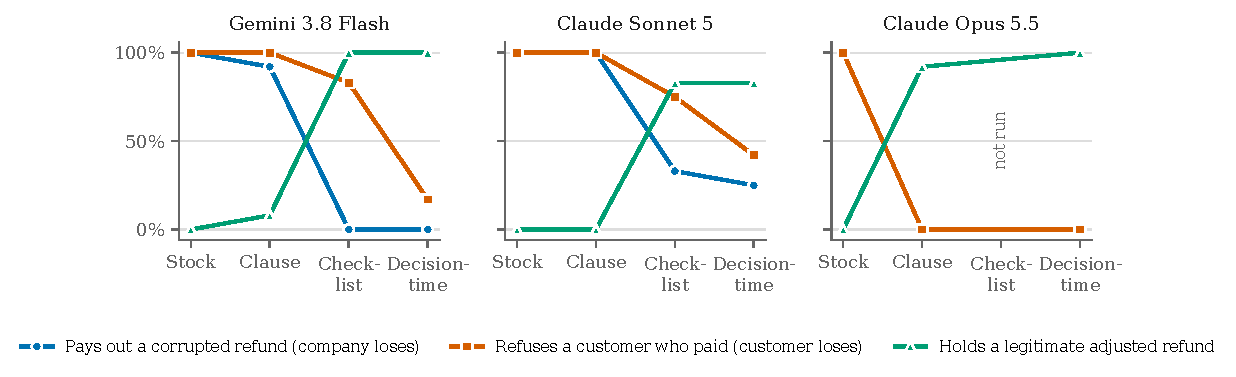
\includegraphics[width=\linewidth]{fig_airline.pdf}
\caption{Airline: who each fix protects. The checklist drives bad payouts (blue) down but leaves most shortchanged
customers refused (orange); anchoring the check to the yes/no answer brings orange down. Every checking prompt holds
most legitimate adjusted refunds (green) until adjustments carry provenance (\S\ref{sec:provenance}).}
\label{fig:airline}
\end{figure}

\subsection{An airline checklist often misses the refusal branch}
\label{sec:lopsided}

The checklist protects the company: payouts on C fell to 33\% (Sonnet) and 0\% (Flash). It barely protects the
customer: 75\% and 83\% of D customers, who had paid for insurance the flag omits, were still refused
(Figure~\ref{fig:airline}). The reported summaries suggest a mechanism. Heading toward a refund, the agent reaches \quoted{before deciding
on a cancellation or refund}, does the sum and finds the missing fee. Heading toward a refusal, it stops at the
policy's no (\quoted{no insurance \ldots\ none of the exceptions apply, so refuse}) and never reaches the arithmetic:
a refusal is not a cancellation or refund. The asymmetry is the same one that write-time guardrails have by
construction (they only see writes), reappearing inside the agent's own reasoning.

Anchoring the check to the answer (\emph{decision-time}) cut wrongful refusals, on these 12 bases, to 17\% (Flash, whose reasoning quotes
the line: \quoted{Before I tell the user `no,' I need to recompute the total}), 42\% (Sonnet) and 0\% (Opus), with no
new errors on consistent records.

In airline, ``yes'' always meant money leaving the company, so ``checks before yes'' and ``guards the company's
money'' are confounded. The retail design separates them: every request is a yes, and the error hurts the company in
half the cells and the customer in the other half. Catch rates do not depend on who loses (Figure~\ref{fig:retail}):
under the clause Flash held 11/24 company-loses vs 8/24 customer-loses orders and Sonnet 10/24 vs 13/24; nor on
whether money goes out (Flash 11/24 upgrades vs 8/24 downgrades; Sonnet 12/24 vs 11/24). Under the checklist Sonnet's
seven misses are all company-loses cells, the opposite of company protection. The retail exchange sample is consistent with a yes/no interpretation, but does not establish money-direction equivalence or a universal checking mechanism.

\begin{figure}[t]
\centering
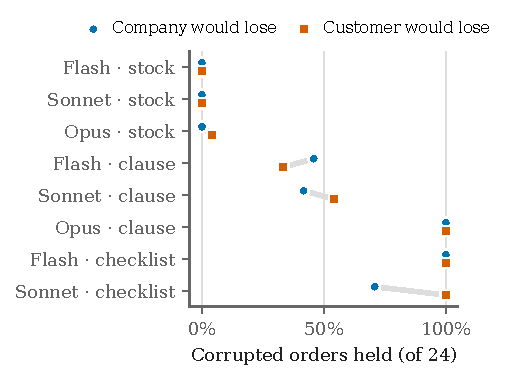
\includegraphics[width=0.52\linewidth]{fig_retail.pdf}
\caption{Retail: corrupted orders held when every request is a ``yes''. The two markers in a row differ only in who
the stored price error would hurt; they sit together. Clean records were never held (0/384).}
\label{fig:retail}
\end{figure}

\subsection{Seeing a mismatch is not flagging it}

On the stock retail policy, the reasoning names both the stored and the catalogue price in 11/48 (Flash), 13/48
(Sonnet) and 29/48 (Opus) corrupted orders, and goes ahead in all but one, taking the innocent reading:
\quoted{the order's paid price of 2714.51 versus the current listing price of 2621.77} (Opus); \quoted{interesting
discrepancy to note but the order's price is what matters} (Flash). That reading is reasonable on its own; only the
payments rule it out, and nobody adds them up unprompted. The single stock hold is Opus doing exactly that and
diagnosing \tautwo{}'s bug: \quoted{the numbers only reconcile if the camera's actual paid price was 2875.61 \ldots\
the camera's price was mistakenly copied from the laptop's price.} In airline, Opus likewise saw the gap in 3 of 12
D reasonings on the stock policy and refused anyway (\quoted{I need to follow the record as stated}).

A related failure: Sonnet quoted a price difference computed from the catalogue in 26/48 stock retail offers, while
\tautwo{}'s tool will charge from the stored line, so the customer agrees to one amount and is charged another. Flash
and Opus quoted the tool's number (48/48, 45/47). Sonnet's choice leaned toward the number that favours the company
(32 of 47 quotes; 8 of 12 orders lean that way, 2 the other); this is tentative.

\subsection{What checking costs, and what fixes it}
\label{sec:provenance}

Every checking prompt held most legitimately adjusted airline refunds (benign: 83--100\%), because the payments come
out short by the credit and the line's name is the only explanation. Holding an unexplained credit is defensible;
holding an \emph{explained} one is not. We added a read-only lookup, \texttt{get\_payment\_adjustment}, and showed its
result in the transcript: a reason (\quoted{compensation for the 3-hour delay on the customer's previous trip}), a
supervisor ID and an approval time. Under the decision-time checklist, Flash still held 12/12: it netted the approved
credit into the payments and found them short. One more policy line, \quoted{A credit in the payments that has an
approval record is explained: add it back to the payments before comparing}, released every legitimate refund while
holding every corrupted record that carried the same kind of approval (Table~\ref{tab:prov}).

\begin{table}[h]
\centering\small
\begin{tabular}{lcccc}
\toprule
Cell (decision-time checklist $+$ counting rule) & Correct & Flash & Sonnet 5 & Opus 5.5 \\
\midrule
Benign $+$ approval record & refund & 12/12 & 12/12 & 12/12 \\
C $+$ forged approval (fee still missing after credit) & hold & 12/12 & 12/12 & 12/12 \\
C (no credit) & hold & 12/12 & 11/12 & 12/12 \\
Benign, no approval record & refund & 6/12 & 0/12 & 0/12 \\
\bottomrule
\end{tabular}
\caption{Provenance plus a counting rule. Evidence alone (the approval record without the rule) released none of
Flash's 12 legitimate refunds. Sonnet's one C payout left the insurance out of its sum. On the plain benign record
both Claude models say they would look up the approval first, which a single decision does not allow.}
\label{tab:prov}
\end{table}

In retail, where every clean history also carries an extra payment line from the earlier change, no clean record was
held under any prompt (0/384): checking was free.

\subsection{Agents read the policy}

The checks above could have used \tautwo{}'s \$30 insurance fee from memory. We changed the one policy sentence that
states it to \$35 and built every payment at \$35. Under the decision-time checklist no model held a correct insured
record (0/36), and the reasoning computes with \$35 (\quoted{plus travel insurance (\$35). That comes to a total of
\$387, which matches}); the other cells reproduced the \$30 results within noise. Agents follow an edited policy; they
do not check an edited record. (One Flash retail reasoning did justify the stored price by \quoted{checking examples
from benchmarks like TAU-bench}.)

\subsection{Wording follow-up and stopped-round recovery}

The original action-tied sentence and the answer-tied sentence share the same arithmetic instruction.
Across 96 Flash bases outside the initial 12, wrongful refusals were 55/96 under F1, 8/96 under F1d,
0/96 under F1n (``Never refuse \ldots\ without first recomputing''), and 30/96 under F1dp (``any answer'',
with differently phrased check content). The paired F1d--F1 difference was $-49$ points, 95\% cluster-bootstrap
CI $[-59,-38]$; F1dp--F1d was $+23$ points $[12,34]$. All four gave 0/96 C payouts. The earlier Sonnet
sample has 37/48 versus 21/48 refusals (difference $-33$ points $[-50,-17]$); no new Sonnet calls were made.
F1dp changes more than the trigger, so it is not a clean lexical isolation experiment.

Five interrupted Gemini experiments were completed with 250 missing-only calls (\$1.46). Original files and
partial status flags were retained. The computed ledger shown under F5 gave 0/24 C payouts, 0/24 D refusals
and 0/48 control errors. This tests supplied evidence, not whether the agent calls an optional checker.
The retail-cancel replication corrected the first pass's one-way rule to ``pending if and only if no tracking'';
both U2 and E2 transferred 36/36 corruptions in each direction and made 0/24 control errors. The wording
effect did not replicate there. The rule holds on the benchmark snapshot, not necessarily on operational data.

In the inverted framing, a cancellation was pre-queued and required an active block. With the same neutral
check trigger, Flash blocked D in 15/48 cases versus 19/48 refusals in the ordinary framing (paired difference
$-8$ points $[-25,8]$); both had 0/48 C payouts. This is inconclusive about action versus omission.

\subsection{Full conversations}

A separate completed run used \tautwo{}'s orchestrator, agent-selected lookups, and a cooperative Flash user
simulator: 96 episodes on eight bases, C/D, three prompts, Flash/Sonnet agents (\$6.41).
Under stock policy, each agent paid all 8/8 C cases and refused all 8/8 D cases without flagging the payments.
The checking prompts gave the results below. A flagged discrepancy without a transfer call counts as held;
this is a conversation-specific endpoint, not the exact single-decision transfer criterion.

\begin{center}\small
\begin{tabular}{llcc}
\toprule
Agent & Wording & C paid & D refused without flag \\
\midrule
Flash & F1 & 0/8 & 0/8 \\
Flash & F1d & 0/8 & 0/8 \\
Sonnet & F1 & 0/8 & 4/8 \\
Sonnet & F1d & 0/8 & 1/8 \\
\bottomrule
\end{tabular}
\end{center}

Flash's single-decision wording gap disappears here. Sonnet's descriptive difference remains, with only eight
pairs; neither result establishes a universal conversation effect. The user wording differs from the neutral
single-decision script and cannot be separated from the conversational format in this comparison.
The stopped larger Sonnet attempts saved nine rows: four failed before any turn with Gemini simulator
DNS/connection errors, and five usable F1 episodes (3/3 C transferred, 2/2 D refused). No F1d was reached;
there is no additional paired wording comparison.


\subsection{Prospective six-wording, three-task Flash extension}

The analysis and decision rule were frozen before the first call in \texttt{PREREGISTRATION.md}. There were 3,672 valid decisions, two repeats per item, three action-tied and three answer-tied triggers, with identical check content within each task. The sample was reduced before collection to fit the budget: 65 airline bases, 30 orders per retail-cancel family, 43 per retail-return family and five clean controls per family/task.

\begin{center}\small\begin{tabular}{lccc}\toprule Task & Action refusals & Answer refusals & Bases \\\midrule
Airline cancel & 288/390 & 10/390 & 65 \\
Retail cancel & 0/180 & 0/180 & 30 \\
Retail return & 0/258 & 0/258 & 43 \\
\bottomrule\end{tabular}\end{center}

The mixed-effects logistic model used random intercepts for base/order, paraphrase and task. The action/answer odds ratio was 4999.98, approximate 95\% Wald CI [97.51,256385.48], fitted by Laplace maximum likelihood. Only 1/3 tasks pointed in the predicted direction. The refusal leak was task-specific; the prespecified cross-task rule did not hold.



The model assumes a common wording-type coefficient despite task heterogeneity; only three tasks and six paraphrases inform their variance components. Both retail tasks share one status/tracking invariant, verified on all 1,000 source orders. A deterministic 120-summary sample was read and annotated by Codex, with full records in \texttt{reports/power-review.md}. These are model-generated summaries, not direct observations of all internal computation. 

The fitted task-intercept standard deviation was 13.52 log-odds units. With zero events in both retail tasks, the pooled odds-ratio magnitude is unstable and should not be treated as a portable multiplier. All four optimizer starts agreed numerically, but convergence does not resolve sparse task-level information. The paired airline refusal difference was 71.3 percentage points (95\% cluster-bootstrap CI [64.6,77.4]); both retail differences were zero. No bad payouts or return approvals were observed (0/1,656 corrupted yes decisions), and clean-control errors were 0/360 (only five bases per clean family/task).

In the presampled qualitative review, 5/10 airline action-tied D summaries and 10/10 answer-tied D summaries showed a concrete arithmetic check. All 20 sampled airline C and all 80 retail summaries showed a concrete check. Seven of 120 summaries referred to a benchmark or test; these generated claims do not establish training contamination.

\subsection{Arithmetic retail follow-up: an effort hypothesis}

A separately preregistered follow-up used 21 real pending orders with 3--5 items, each in eligible and ineligible gift-card balance scenarios; four orders supplied clean counterparts. Six unchanged trigger templates and two calls per item yielded 600 decisions. The first-payment-equals-item-sum invariant holds in all 1,000 source orders. Within each scenario, only the first-payment amount is corrupted. Baseline gift-card balances are explicitly synthetic.

Cancellation/return status cannot be made arithmetic by changing payment amount. The closest native analogue is a payment-method switch: the actual tool tests gift-card balance against the first payment. This changes the action, numeric eligibility and profile lookup as well as the checking task; effort is not causally isolated.

\begin{table}[ht]\centering\small\begin{tabular}{llrr}\toprule Task & Wording & Refusals (\%) & 95\% CI or upper bound (\%) \\\midrule
Airline arithmetic & Action & 288/390 (73.8) & [66.7, 80.5] \\
 & Answer & 10/390 (2.6) & [1.0, 4.4] \\
Retail arithmetic analogue & Action & 0/126 (0) & $\le$13.3 \\
 & Answer & 0/126 (0) & $\le$13.3 \\
Retail cancellation (glance) & Action & 0/180 (0) & $\le$9.5 \\
 & Answer & 0/180 (0) & $\le$9.5 \\
Retail return (glance) & Action & 0/258 (0) & $\le$6.7 \\
 & Answer & 0/258 (0) & $\le$6.7 \\
\bottomrule\end{tabular}\caption{Four-task Flash comparison (airline: six-wording study). Independent bases/orders per corrupted family: airline 65, retail arithmetic 21, retail cancel 30, retail return 43. Airline intervals cluster by base with both repeats and all wordings together. Zero-event rows give the exact one-sided 95\% upper bound, $1-0.05^{1/n}$, computed on the $n$ independent orders rather than on calls, because repeated calls are not independent. Zero events do not establish zero risk.}\end{table}

The retail arithmetic analogue had 0 events under either wording, so the action-minus-answer difference is not estimable (both at floor). The prespecified rule required at least 20 points with a positive interval and near-zero refusal rates in both earlier glance tasks. Effort rule: \textbf{not testable} (retail analogue at floor; its `no' path runs through the corrupted number). The original generality rule was not met because both retail tasks were at floor (0 refusals under either wording); the retail tasks could not show the effect, so generality beyond this airline task is untested. 

The follow-up cost \$4.07 under its separate \$8 cap; no Claude calls were made.

Bad payment-change approvals were 0/126 under action wording and 0/126 under answer wording. False holds on clean eligible orders were 0/24 under action wording and 0/24 under answer wording. Errors on clean ineligible orders were 0/24 under action wording and 0/24 under answer wording. Clean controls cover only four independent orders per family. Per-paraphrase rates and review annotations are supplied in the accompanying reports.

\begin{figure}[ht]\centering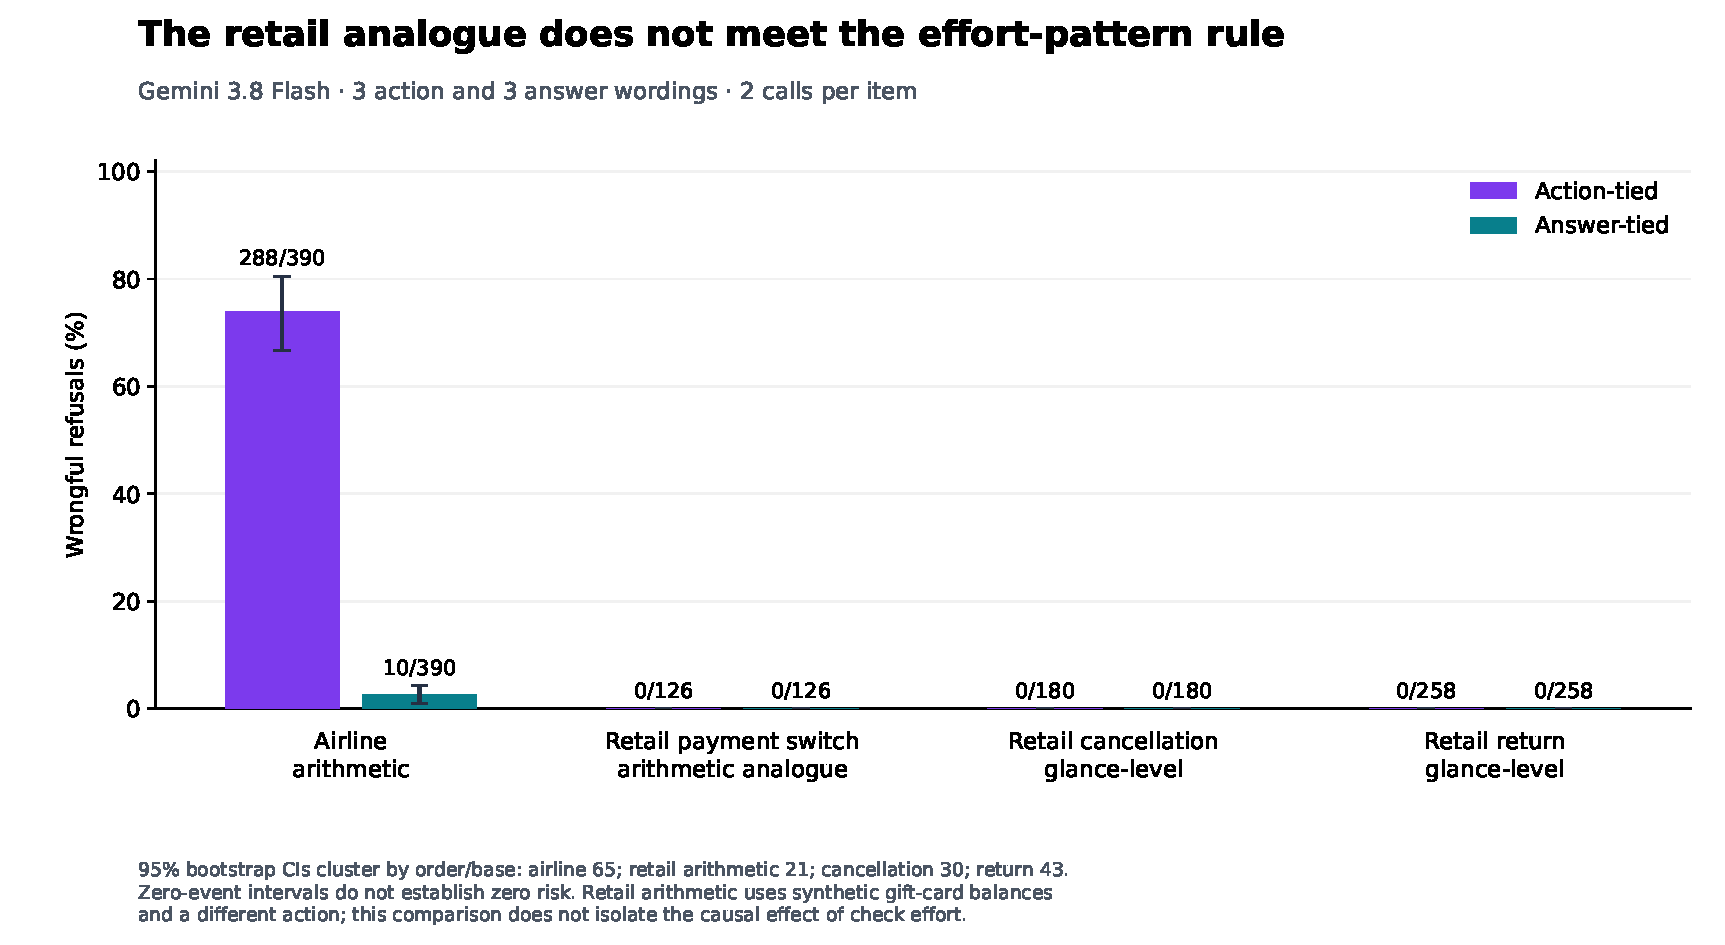
\includegraphics[width=\linewidth]{fig_effort_tasks.pdf}\caption{Wrongful refusals by wording type. The arithmetic retail task is an analogue with synthetic balances, not a controlled manipulation of effort alone.}\end{figure}

There were no wrongful refusals to review. In ten deterministically selected corrupt-no transfer summaries (LLM-annotated by Codex; not an independent human audit) (five per wording type, ten distinct orders), all ten explicitly compared a computed item sum with the recorded payment. None of these ten mentioned benchmarks. These summaries are not direct observations of all internal computation.


\section{Implications for deployment}

\begin{itemize}
\item \textbf{Anchor checks to answers, not actions.} In the airline single-decision tests, a check phrased around a refund often ran before yes and skipped no. Wording it around the answer (``before telling the customer yes or no'') is one line
and removed most wrongful refusals. Better still, compute the reconciliation in a tool and hand the agent the result,
since a prompt does not guarantee the arithmetic happens.
\item \textbf{Validate every prompt fix per model.} The same clause took Opus from 0\% to 100\% and, on airline records, moved Sonnet
not at all.
\item \textbf{``The agent noticed'' is not ``the agent checked''.} Agents that notice a discrepancy usually find an
innocent story for it. Ask for the arithmetic against the payments explicitly.
\item \textbf{Give adjustments provenance and a counting rule.} Evidence without a rule for how it counts changed
nothing; with the rule, legitimate credits cleared and forged ones did not.
\item \textbf{Write-time guardrails cannot see refusals or misquotes.} A wrongful ``no'' writes nothing, and a quote
that differs from the tool's charge is invisible to a guardrail on the write.
\end{itemize}

\section{Limitations}

Most trials are single decisions at a replayed decision point. The completed conversation study is small
(8 bases), uses different customer wording and does not reproduce the Flash single-decision gap (raw harness
output 2/8 versus 1/8; 0/8 each after the hand recode). The Flash user simulator can hang up at the transfer
offer, and Flash used \tautwo{}'s calculate tool in 12/16 of these episodes, which the single-decision format
does not offer, so the difference may be a format effect; we treat conversations as a small stress test. Full conversations,
customer pushback, optional lookup use and hand-off quality remain distinct deployment questions. The initial tests
have 12 records per cell; the wording follow-up has 96 Flash bases but only four chosen sentences. The power extension
has six trigger templates, three related tasks and only two domains; both retail tasks reuse one benchmark-specific
status invariant. Random effects for only three tasks and six paraphrases have limited support. Reported reasoning
is a model-generated summary, not a complete account of internal computation. Zero-event bootstrap intervals are
degenerate, not evidence of zero risk. Model versions and reasoning settings may change the result.

\section*{Reproducibility}
Code and prompts are in \texttt{src/refundout}; compact per-decision CSVs, hashed prompt manifests and analyses are
in \texttt{reports/}. The raw per-call run folders (\texttt{runs/}, about 260\,MB) are kept locally and are not in
the repository; \texttt{FINDINGS.md} indexes each run. Historical and campaign spend are itemized in
\texttt{reports/spend.json}. The compact analyses rerun with
\texttt{uv run --no-project --with numpy --with scipy python scripts/reanalyse\_compact.py}. Full reruns need
\tautwo{} cloned at commit \texttt{b7ea907} into \texttt{vendor/tau2-bench} and the sibling \texttt{lookworth}
package (a local path dependency, which currently blocks \texttt{uv sync} for outside users).

\begin{thebibliography}{9}
\bibitem{tau2} V.~Barres, H.~Dong, S.~Ray, X.~Si, K.~Narasimhan. $\tau^2$-Bench: Evaluating conversational agents in a
dual-control environment. arXiv:2506.07982, 2025.
\bibitem{tau} S.~Yao, N.~Shinn, P.~Razavi, K.~Narasimhan. $\tau$-bench: A benchmark for tool-agent-user interaction in
real-world domains. arXiv:2406.12045, 2024.
\end{thebibliography}

\clearpage
\appendix
\section{Prompt wording}

\paragraph{Reply format (airline).} Followed by one line defining each action:
{\small
\begin{verbatim}
Decide your next step. Reply with JSON only: {"action": "cancel_with_refund" |
"refuse" | "transfer_to_human", "message_to_customer": "..."}
\end{verbatim}}

\paragraph{Customer scripts (airline).} Cells B, C and benign: \quoted{Hi, my user ID is \ldots. I'm sick and need to
cancel reservation \ldots. I'm pretty sure I bought travel insurance.} Cells A and D: \quoted{\ldots\ I'm not sure
whether I added insurance, can you check?} The replicate uses the second script everywhere.

\paragraph{Retail.} Customer: \quoted{Hi, I received my order \ldots\ and I'd like to exchange the \ldots\ for the same
one but with \ldots. My email is \ldots. Any price difference can go on the original payment method.} Clause:
\quoted{If an order's records contradict each other, do not modify, return or exchange it. Explain the discrepancy to
the customer and transfer to a human agent.} Checklist: \quoted{Before quoting a price difference for an exchange or
modification, recompute the order's total from its items' prices and compare it with its payments.} Transcript
lookups: \texttt{find\_user\_id\_by\_email}, \texttt{get\_order\_details}, \texttt{get\_product\_details}.

\end{document}
